\section{Algorithmic construction}
\label{app:algorithm}

We specify the randomized sampler $\RandomizedPackedSampler$ of
Theorem~\ref{app:thm:finite-upper}, also denoted
$\PackedSampler:=\RandomizedPackedSampler$.
All operations use only public parameters, the realized commit history, and
replies of the single frozen oracle.  The hidden forest, exact marginals,
endpoint kernels, ranks, and response witnesses are never read.

The sampler flow in \cref{fig:algorithm-overview-20260918} is illustrated
concretely by a $15$-vertex construction in
\cref{ex:algorithm-banks-20260918,ex:algorithm-submissions-20260918,ex:algorithm-peel-centroids-20260918}.

\subsection{Complete sampler and public parameters}
\label{app:algorithm-overview}
\label{app:algorithm-complete-sampler}

We assemble the sampler from read-only screens and commits, with public
caps that bound its execution on every path.

Fix $N\ge10$.  The two resource controls are the degree cutoff
$\DegreeCutoff\in\{9,\ldots,N-1\}$ and readout-chunk parameter
$\ChunkCount\in\PositionSet$: the former sets the peeling threshold, while
the latter sets the maximum readout size
$\ReadoutChunkSize:=\lceil N/\ChunkCount\rceil$.
The accuracy inputs are a tail tolerance $\TailTolerance\in(0,1]$ and a
screen-failure budget $\ScreenFailureBudget\in(0,1)$.
The threshold floor $\ThresholdFloor$ uses the standard choice
\eqref{app:eq:rate-threshold-floor}.
The draft generator is the zero-query choice
\eqref{app:eq:standard-draft} unless otherwise stated.
The standard row selector keeps the highest-vote candidates on overflow.
More generally, fix any admissible public selector $\RowSelector$ from
Definition~\ref{app:def:row-selector}; denote the resulting decision rule by
$\SelectedPackedSampler$.  The unadorned sampler uses the standard selector.
The row-error radius and resulting screen resolution are derived quantities:
\begin{align}
 \RowTVError&:=\frac{\OracleRadius}{\sqrt N},
 \label{app:eq:oracle-tv-radii}\\
 \ScreenResolution&:=4\RowTVError+\TailTolerance.
 \label{app:eq:diameter-screen-resolution}
\end{align}
The oracle condition \eqref{app:eq:A2} and
\cref{app:lem:finite-hellinger-calculus} imply, for every valid $(y,j)$,
\begin{equation}
 \dTV\bigl(\ExactRow{y}{j},\OracleRow{y}{j}\bigr)
 \le\RowTVError.
 \label{app:eq:oracle-tv-radius}
\end{equation}
\textcolor{red}{The preprocessing and screen certificates use the row-TV bound
\eqref{app:eq:oracle-tv-radius} in both cases.  In \KLCase,
\eqref{app:eq:kl-oracle-inclusion} supplies this bound from the uniform
forward row-KL condition.  The forward-KL output guarantee is proved in
\cref{app:thm:finite-kl-upper} using the joint-reference identity of
\cref{app:kl-joint-reference}.}
The theorem requires feasible preprocessing and
$\ScreenResolution<\EdgeSignal$; neither condition asks the sampler to inspect
the hidden forest.

Define the public peel-phase cap
\begin{equation}
 \PeelPhaseCap
 :=\left\lceil
 \frac{\PositivePart{\log(2N/(\DegreeCutoff+1))}}
      {\log(\DegreeCutoff/8)}
 \right\rceil.
 \label{app:eq:phase-cap}
\end{equation}
Set
\begin{equation}
 \ScreenCallCap:=\PeelPhaseCap+1,
 \qquad
 \HardRoundCap
 :=\left\lceil\frac{4N\PeelPhaseCap}{\DegreeCutoff}\right\rceil
   +\left\lceil\log_2(N+1)\right\rceil+2.
 \label{app:eq:screen-call-and-round-caps}
\end{equation}
The caps are fixed before the first commit; they are not additional tuning
parameters.  Algorithm~\ref{app:alg:complete-sampler} is the full decision rule.
Its one-time preprocessing, per-screen draft, and read-only screen are
specified in the next three subsections.
The named steps agree with Section~\ref{sec:main-algorithm} and
Figure~\ref{fig:algorithm-overview-20260918}.
Their identifiers name recurring operations, not commit rounds or oracle stages.
\AlgoBlockRef{screen} is expanded into
\AlgoBlockRef{chunks}, \AlgoBlockRef{probes}, and \AlgoBlockRef{aggregate}
in Algorithm~\ref{app:alg:packed-screen}.
Proofs refer to these named steps as well as the algorithm's line numbers.
In Algorithm~\ref{app:alg:complete-sampler}, $r$ counts completed nonempty
commit rounds and $k$ counts completed peel phases.

% Please keep the full sampler on one float page without blocking the preceding text.
\begin{algorithm}[p]
\caption{Randomized complete packed-screen sampler}
\label{app:alg:complete-sampler}
\begin{algorithmic}[1]
\Require the public setup and parameters
  $\TailTolerance,\ThresholdFloor,\DegreeCutoff,\ChunkCount$,
  $\ScreenFailureBudget$, an admissible $\DraftGenerator$ (standard by default),
  an admissible public row selector $\RowSelector$ (top votes by default),
  and access to $\FrozenOracle$
\Ensure $\SamplerOutput\in\Vocab^N$ when preprocessing is feasible; otherwise
  \InfeasibleOutcome
\Statex \AlgoBlockTarget{preprocess}
\State Construct $\PreprocessData$ by Definition~\ref{app:def:preprocessing}
\If{preprocessing reports infeasibility}
  \State \Return \InfeasibleOutcome
\EndIf
\State Set $\ScreenCallCap,\HardRoundCap$ by
  \ref{app:eq:screen-call-and-round-caps} and set
  $G\gets\emptyset$, $x_G\gets\emptyset$, $k\gets0$, and $r\gets0$
\Loop
  \If{$\ResidualPositions=\emptyset$}
    \State \Return the resulting assignment $\SamplerOutput$
  \EndIf
  \Statex \AlgoBlockTarget{draft}
  \State Fix $\DraftFiller\gets\DraftGenerator$ using the current history and past replies
  \State Draw the coloring family by \eqref{app:eq:random-color-draw},
    with parameters from \eqref{app:eq:random-color-parameters}
  \Statex \AlgoBlockTarget{screen}
  \State $\ScreenRows\gets
    \Call{\PackedScreenName}{\History;\PreprocessData,\DraftFiller,
      \ColorSet,(\ColorHash{\tau}{\cdot})_{\tau\in\ColoringIndexSet},
      \DegreeCutoff,\ChunkCount,\FrozenOracle,\RowSelector,\ScreenTranscript}$
    \Comment{\cref{app:alg:packed-screen}}
  \Statex \AlgoBlockTarget{peel}
  \State Form $\ClaimCount{\cdot}$ and $\PeelSet$ by
    \ref{app:eq:claim-and-peel-set}
  \If{$\PeelSet=\emptyset$ or $k=\PeelPhaseCap$}
    \State \textbf{break}
  \EndIf
  \State Freeze $\FrozenPeelSet\gets\PeelSet$
  \For{$v\in\FrozenPeelSet$ in increasing position order}
    \If{$r=\HardRoundCap-1$} \Comment{\AlgoGuardRef}
      \State $\Call{\CommitName}{\ResidualPositions}$ and
        $r\gets r+1$
      \Return the resulting assignment $\SamplerOutput$
    \EndIf
    \State $\Call{\CommitName}{\{v\}}$
    \State $r\gets r+1$
  \EndFor
  \State $k\gets k+1$
\EndLoop
\Statex \AlgoBlockTarget{terminal}
\State $\TerminalHistory\gets\History$,
  $\TerminalPositions\gets\ResidualPositions$, and
\Statex \hspace{\algorithmicindent}$\displaystyle
 \CertifiedEdges\gets
 \{\{u,v\}\subseteq\TerminalPositions:
 v\in\ScreenRowAt{\TerminalHistory}{u}
 \text{ or }u\in\ScreenRowAt{\TerminalHistory}{v}\}$
\State $\CertifiedForest\gets(\TerminalPositions,\CertifiedEdges)$
\While{$\CertifiedForest$ contains a cycle}
  \If{$r=\HardRoundCap-1$} \Comment{\AlgoGuardRef}
    \State $\Call{\CommitName}{\ResidualPositions}$ and $r\gets r+1$; \Return $\SamplerOutput$
  \EndIf
  \State Choose a maximum-degree cycle vertex $v$; break ties by smallest index
  \State $\Call{\CommitName}{\{v\}}$; $r\gets r+1$; delete $v$ and its incident edges from $\CertifiedForest$
\EndWhile
\Statex \AlgoBlockTarget{centroid}
\While{$\CertifiedForest$ has a vertex}
  \State In each component choose its smallest-label centroid; call their set $B$
  \If{$r=\HardRoundCap-1$} \Comment{\AlgoGuardRef}
    \State $\Call{\CommitName}{\ResidualPositions}$ and
      $r\gets r+1$
    \Return the resulting assignment $\SamplerOutput$
  \EndIf
  \State $\Call{\CommitName}{B}$
  \State $r\gets r+1$
  \State Delete $B$ and its incident edges from $\CertifiedForest$
\EndWhile
\State \Return the resulting assignment $\SamplerOutput$
\end{algorithmic}
\end{algorithm}

Given the screen output at $\History$, recall the incoming claim count and
peel set of \textcolor{red}{\cref{main:eq:claim-and-peel-set}}:
\begin{equation}
 \ClaimCount{v}
 :=\bigl|\{u\in\ResidualPositions:v\in\ScreenRow{u}\}\bigr|,
 \qquad
 \PeelSet:=\{v\in\ResidualPositions:
             \ClaimCount{v}>\DegreeCutoff/2\}.
 \label{app:eq:claim-and-peel-set}
\end{equation}
\textcolor{red}{The terminal row graph on $\TerminalPositions$ is constructed in
\AlgoBlockRef{terminal} of \cref{app:alg:complete-sampler}.}

At any history, $\CommitOperation(B)$ means the product-commit operation
of Definition~\ref{app:def:admissible-algorithm}: submit the current
history-compatible commit state \ref{app:eq:commit-state}, read
$\OracleRow{y}{j}$ for $j\in B$, draw independently from the corresponding
product law, and append the realized values to the history.  This is the
sampler's only history-changing operation. The batch $B$ is fixed before
the reply; this submission adds one to $\CommitRounds$ and nothing to
$\CounterfactualQueries$.

\begin{enumerate}
 \item \emph{Screen, then test whether to stop.}
 Each pass first computes rows at the current history
 (\AlgoBlockRef{screen}) and only then tests whether the peel set is empty
 or the phase cap has been reached (\AlgoBlockRef{peel}).
 In particular, the last permitted peel phase is followed by another
 screen: the terminal graph never uses rows from before those commits.
 A nonempty peel set is frozen before its singleton commits; its members
 are committed in position order, without an intervening screen or
 recomputation of that set.

 \item \emph{Repair cycles in the terminal estimate.}
 In \AlgoBlockRef{terminal}, the working graph $\CertifiedForest$ initially
 equals $(\TerminalPositions,\CertifiedEdges)$. A cycle vertex belongs to
 at least one simple cycle of this graph. The selection rule is
 \[
 v=\min\operatorname*{arg\,max}_{
       \substack{u\in V(\CertifiedForest)\\
                 u\text{ lies on a cycle of }\CertifiedForest}}
       d_{\CertifiedForest}(u).
 \]
 The degree is measured in the whole current working graph.
 Commit $v$ using the current history, delete $v$ and its incident edges,
 and recompute cycle membership and degrees in the remaining graph.
 No new screen is run: the graph changes only by vertex deletion, whereas
 each commit queries fresh rows at the updated history.
 Once it is a forest, proceed to \AlgoBlockRef{centroid}.

 \item \AlgoGuardTarget.
 Before each peel, repair, or centroid commit, the check
 $r=\HardRoundCap-1$ reserves the last permitted round for one product
 commit of all remaining positions. This ends the execution even if
 repair is incomplete. The cap bounds the round count on every path;
 this final product law need not approximate the true joint conditional.

 \item \emph{Separate the observable past from the random sources.}
 All ties use the public position or token order.
 The public transcript $\ScreenTranscript$ starts with preprocessing
 and is updated after each query, coloring draw, selector output, and
 commit. It records only information already available to the decision
 rule, not unrevealed future randomness.
 The decision-rule seed $\ControllerSeed$ contains the coloring blocks
 and auxiliary draft randomness. Product-commit draws use a separate
 random source: even after conditioning on $\ControllerSeed=w$, those
 draws remain random and are integrated into
 $\SamplerOutputLaw{w}{\FrozenOracle}$.
\end{enumerate}

\subsection{One-time all-mask preprocessing}
\label{app:algorithm-preprocessing}

In \AlgoBlockNamedRef{preprocess}, one all-mask submission supplies the
local vocabulary banks $\TokenBank{i}$ and tail representatives
$\TailRepresentative{i}$ reused by every later screen.

\begin{definition}[All-mask preprocessing]
\label{app:def:preprocessing}
Use the standard floor
\begin{equation}
 \ThresholdFloor:=\StandardThresholdFloor{\FrequencyConstant}.
 \label{app:eq:rate-threshold-floor}
\end{equation}
Here $\FrequencyConstant\ge1$ is the public RF\textcolor{red}{~(\cref{app:eq:RF})} constant when an envelope is
specified; otherwise use $\FrequencyConstant=1$.
This keeps the threshold above both the row-noise and
frequency-envelope scales.
If $\ThresholdFloor>1$, return $\InfeasibleOutcome$.
Otherwise put
$\ThresholdGridDepth:=\lceil\log_2(1/\ThresholdFloor)\rceil$ and set
\begin{equation}
 \ThresholdGrid
 :=\{\max\{\ThresholdFloor,2^{-m}\}:0\le m\le\ThresholdGridDepth\}.
 \label{app:eq:threshold-grid}
\end{equation}
Form the feasible set
\begin{equation}
 \FeasibleThresholdGrid
 :=\{t\in\ThresholdGrid:
       \min\{1,\ResponseConstant t^{\ResponseExponent}\}\le\TailTolerance\}.
 \label{app:eq:feasible-threshold-grid}
\end{equation}
If it is empty, return $\InfeasibleOutcome$ before any submission or commit.
Otherwise set $\TailThreshold:=\max\FeasibleThresholdGrid$.

Submit $\AllMaskState=(\MASK,\ldots,\MASK)$ once and, for each position $i$,
form its noisy marginal and \emph{local vocabulary bank}:
\begin{align}
 \NoisyMarginal{i}&:=\OracleRow{\AllMaskState}{i},
 \label{app:eq:noisy-marginal}\\
 \TokenBank{i}
 &:=\{a\in\Vocab:\NoisyMarginal{i}(a)\ge\TailThreshold-\RowTVError\}.
 \label{app:eq:local-bank}
\end{align}
Here $\TokenBank{i}\subseteq\Vocab$ is the subset of vocabulary tokens
selected by the buffered all-mask marginal threshold
$\TailThreshold-\RowTVError$ for explicit source-value probing.
Tokens outside this set are represented in the response test by
$\TailRepresentative{i}$ below; the set does not restrict commit outputs.
Enumerate the vocabulary bank $\TokenBank{i}$ as
$\TokenBank{i}=\{\BankToken{i}{1},\ldots,\BankToken{i}{\BankSize{i}}\}$
in the public token order, with $\BankSize{i}:=|\TokenBank{i}|$ and
$\MaxBankSize:=\max_i\BankSize{i}$, and choose
\begin{equation}
 \TailRepresentative{i}:=
 \min_{\TokenOrder}\bigl(\Vocab\setminus\TokenBank{i}\bigr).
 \label{app:eq:positionwise-baseline}
\end{equation}
The floor ensures that this complement is nonempty;
\cref{app:lem:preprocessing-certificates} proves both existence and its
exact-tail certificate.  Return the reusable tuple
\begin{equation}
 \PreprocessData:=
 \left(\TailThreshold,
 (\NoisyMarginal{i},\TokenBank{i},\TailRepresentative{i},\BankSize{i})_{i\in\PositionSet},
 \MaxBankSize\right).
 \label{app:eq:preprocessing-output}
\end{equation}
Apart from the all-mask submission, preprocessing is deterministic and uses
no commit draw.
\end{definition}

\subsection{Per-screen draft and source columns}
\label{app:algorithm-draft}

We first fix the common background for one screen, then define the source
assignments whose oracle replies will be compared.

\begin{example*}[Standard zero-query draft]
Unless stated otherwise, \AlgoBlockRef{draft} uses the standard draft
\begin{equation}
 \DraftToken{i}
 :=\mathop{\arg\max}_{a\in\Vocab}\NoisyMarginal{i}(a),
 \qquad i\in\ResidualPositions,
 \label{app:eq:standard-draft}
\end{equation}
with ties resolved by $\TokenOrder$.  It reuses the initial all-mask rows,
works even for empty vocabulary banks, and requires no additional submission or adaptive
stage.
\end{example*}

\paragraph{Source columns.}
For the source assignments in \AlgoBlockRef{probes}, recall that
$\TokenBank{i}=\{\BankToken{i}{1},\ldots,\BankToken{i}{\BankSize{i}}\}$
lists the local vocabulary bank in the public token order, not in
marginal-probability order.
Here $\BankSize{i}=|\TokenBank{i}|$ and
$\MaxBankSize=\max_{i\in\PositionSet}\BankSize{i}$ were fixed by preprocessing.
For a fixed screen draft, set
\begin{equation}
 \ScreenColumnSet:=[\MaxBankSize]\cup\{\TailColumn\},
 \qquad
 \PackedColumn{\kappa}{i}
 :=\begin{cases}
 \BankToken{i}{\kappa},&\kappa\in[\BankSize{i}],\\
 \DraftToken{i},&\kappa\in[\MaxBankSize]\setminus[\BankSize{i}],\\
 \TailRepresentative{i},&\kappa=\TailColumn.
 \end{cases}
 \label{app:eq:packed-column}
\end{equation}
The column order is $1,\ldots,\MaxBankSize,\TailColumn$.
Thus a bank-column index denotes a position-dependent assignment, not one
common vocabulary token.  All screen quantities below depend on the fixed
$\DraftFiller$; this dependence is suppressed in row-family, vote, and graph
notation.  When $\MaxBankSize=0$, the screen returns empty rows without
submitting even the tail column.

For resource accounting, the number of submitted columns is
\begin{equation}
 \ScreenColumnCount:=
 \begin{cases}
 \MaxBankSize+1,&\MaxBankSize\ge1,\\
 0,&\MaxBankSize=0.
 \end{cases}
 \label{app:eq:screen-column-count}
\end{equation}

\begin{example}[A column indexes local vocabulary banks, not a common token]
\label{ex:algorithm-banks-20260918}
Take $N=15$, $G=\emptyset$, and a vocabulary whose first three tokens in
the public order are $a\prec b\prec c$ (further tokens may follow).
Suppose the local vocabulary banks $\TokenBank{i}$ from
\AlgoBlockRef{preprocess} (\cref{app:def:preprocessing}) and the fixed draft are
\[
 \TokenBank{1}=\{a,c\},\quad \DraftToken{1}=a,
 \qquad
 \TokenBank{i}=\{b\},\quad \DraftToken{i}=b
 \quad (i\in[15]\setminus\{1\}).
\]
This specifies the screen inputs, not a target distribution or an oracle.
In particular, $\BankSize{1}=2$, $\BankSize{i}=1$ for $i\ne1$, and
$\MaxBankSize=2$.  The first token outside each bank is
$\TailRepresentative{1}=b$ and $\TailRepresentative{i}=a$ for $i\ne1$.
Substituting into \eqref{app:eq:packed-column} gives
\[
\begin{array}{c|ccc}
 \text{position}&\kappa=1&\kappa=2&\kappa=\TailColumn\\ \hline
 1& a&c&b\\
 i\ne1&b&\DraftToken{i}=b&a
\end{array}
 \qquad
 \ScreenColumnSet=\{1,2,\TailColumn\},\quad \ScreenColumnCount=3.
\]
Thus column $1$ assigns $a$ at position $1$ but $b$ at position $4$.
Column $2$ uses the second bank token at position $1$ and draft padding
at position $4$, whose bank has no second token.  The tail column uses
the representative outside each bank.  The same three columns are
reused for every source color and readout chunk.
\end{example}

% Please keep color labels distinct from the source-column index.
\paragraph{Three different indices.}
The screen uses the following roles; their domains and sampling law are
specified in \cref{app:algorithm-screen}.
\par\smallskip
\noindent
\begin{tabularx}{\linewidth}{@{}lXX@{}}
\toprule
Symbol & What it selects & What it does not select\\
\midrule
$\tau$ & One entire coloring $h_\tau:\PositionSet\to\ColorSet$
       & A color within that coloring\\
$c^{\mathrm{src}},c^{\mathrm{rd}}$
       & Source and readout colors under the chosen $h_\tau$
       & Vocabulary tokens\\
$\kappa\in\ScreenColumnSet$
       & One slot in the vocabulary bank $\TokenBank{i}$ or its tail representative,
         separately at each source $i$
       & A color or one common token\\
\bottomrule
\end{tabularx}
\par\smallskip
Thus fixing $\tau$ fixes all position colors; fixing $c^{\mathrm{src}}$
then fixes which residual positions are sources. Varying $\kappa$
changes the tokens assigned to those sources, without recoloring them.
The concrete substitution into the submitted-state definition is in
\cref{ex:algorithm-submissions-20260918}.


\begin{definition}[Zero-query screen draft]
\label{app:def:draft-generator}
Before each screen, $\DraftGenerator$ fixes a token vector
$\DraftFiller\in\Vocab^{\ResidualPositions}$ using only public data,
the realized history, cached oracle replies, and auxiliary seed randomness
independent of the coloring and product-commit random sources. It terminates
without a submission or commit and without observing current or future
colors. The draft is fixed across all colorings, chunks, source colors,
and columns of this screen; it may be reused or changed at the next screen.
A draft token $\DraftToken{i}$ need not belong to the vocabulary bank
$\TokenBank{i}$ and is never committed directly.
\end{definition}

\subsection{Packed randomized-color screen}
\label{app:algorithm-screen}

We generate one color family, pack its readouts into chunks, and compare
source-column replies to form the screen's neighbor claims.

\paragraph{Random color generation.}
For \AlgoBlockRef{draft}, set
\begin{equation}
 \RandomColorCount:=8(\DegreeCutoff+1),
 \qquad
 \RandomColoringCount
 :=\left\lceil
 8\log\frac{\ScreenCallCap N^2}{\ScreenFailureBudget}
 \right\rceil.
 \label{app:eq:random-color-parameters}
\end{equation}
Write $\ColorCount=\RandomColorCount$,
$\ColoringCount=\RandomColoringCount$,
$\ColorSet=[\ColorCount]$, and $\ColoringIndexSet=[\ColoringCount]$.
These are deterministic public parameters.
At each reached screen $s$, conditional on the realized past including its
completed draft, the decision rule reveals a fresh block $W_s$ with law
\begin{equation}
 \ColorHash{\tau}{i}
 \overset{\mathrm{i.i.d.}}{\sim}\operatorname{Unif}([\ColorCount]),
 \qquad
 (\tau,i)\in[\ColoringCount]\times\PositionSet.
 \label{app:eq:random-color-draw}
\end{equation}
The blocks $(W_s)_{s\le\ScreenCallCap}$ are mutually independent and independent
of the auxiliary draft random source and primitive commit randomness;
no current or future block is revealed during draft generation.
The same family is used for all chunks, source colors, and columns of this
screen: \cref{app:alg:packed-screen} does not draw or refresh colors.

\paragraph{Accuracy calibration for the main benchmarks.}
The choices $\ScreenFailureBudget=\OracleRadius/2$ in \HellingerCase\
and $\ScreenFailureBudget=\KLTargetTolerance/(2N\log\VocabSize)$ in
\KLCase\ specialize \eqref{app:eq:random-color-parameters} to
\begin{equation}
 \RandomColorCount=8(\DegreeCutoff+1),
 \qquad
 \RandomColoringCount
 :=\begin{cases}
 \displaystyle\left\lceil
 8\log\frac{2\ScreenCallCap N^2}{\OracleRadius}
 \right\rceil,&\text{\HellingerCase},\\[6pt]
 \displaystyle\left\lceil
 8\log\frac{2\ScreenCallCap N^3\log\VocabSize}{\KLTargetTolerance}
 \right\rceil,&\text{\KLCase}
 \end{cases}
 \label{app:eq:accuracy-color-parameters}
\end{equation}
In \KLCase, all radius-dependent preprocessing and screen quantities use
$\KLOracleRadius$ in place of $\OracleRadius$,
as in \cref{app:cor:kl-epsilon}. The decision rule and commit rule
are unchanged.

\paragraph{Readout chunks.}
Given the colors, \AlgoBlockRef{chunks} partitions each readout class
deterministically so that
each probe masks at most $\ReadoutChunkSize$ positions.
For every $\tau\in\ColoringIndexSet$ and
$\ReadoutColorValue\in\ColorSet$, let
\begin{equation}
 \ColorClass{\tau}{\ReadoutColorValue}
 :=\{j\in\ResidualPositions:
      \ColorHash{\tau}{j}=\ReadoutColorValue\},
 \qquad
 \ColorClassSize{\tau}{\ReadoutColorValue}
 :=|\ColorClass{\tau}{\ReadoutColorValue}|.
 \label{app:eq:color-class}
\end{equation}

For a nonempty class, put
$n:=\ColorClassSize{\tau}{\ReadoutColorValue}$, list its elements in increasing
position order as
$j_{\tau,\ReadoutColorValue,1}<\cdots<j_{\tau,\ReadoutColorValue,n}$, and
partition it into
\begin{equation}
 \ReadoutChunk{\tau}{\ReadoutColorValue}{m}
 :=\left\{
 j_{\tau,\ReadoutColorValue,\ell}:
 (m-1)\ReadoutChunkSize<\ell\le
 \min\{m\ReadoutChunkSize,n\}
 \right\},
 \quad
 1\le m\le\left\lceil
 \frac{n}{\ReadoutChunkSize}
 \right\rceil.
 \label{app:eq:readout-chunks}
\end{equation}
Empty color classes create no chunk.  The chunks depend on the current
residual set $\ResidualPositions$, form a disjoint cover of each color class,
and have size at most $\ReadoutChunkSize$.  Write $\ReadoutChunkOf{\tau}{j}$ for the unique chunk containing $j$.

\paragraph{Submitted states.}
In \AlgoBlockRef{probes}, each probe masks one readout chunk and changes
one source color's
assignment, while keeping the remaining background fixed.
For a nonempty readout chunk
$\mathcal C=\ReadoutChunk{\tau}{\ReadoutColorValue}{m}$,
$\kappa\in\ScreenColumnSet$, and a source color
$\SourceColorValue\in
\ColorSet\setminus\{\ReadoutColorValue\}$, define the probe state
\begin{equation}
 (\ProbeState{\kappa}{\tau}{\SourceColorValue}{\mathcal C})_k
 :=\begin{cases}
 x_k,&k\in G,\\
 \MASK,&k\in \mathcal C,\\
 \PackedColumn{\kappa}{k},
   &k\in\ResidualPositions\setminus \mathcal C\text{ and }
    \ColorHash{\tau}{k}=\SourceColorValue,\\
 \DraftToken{k},&\text{otherwise}.
 \end{cases}
 \label{app:eq:screen-probe-state}
\end{equation}
Here $\ReadoutColorValue$ is the readout color,
$\SourceColorValue$ is the source color, and $\tau$ selects the entire
coloring.  Since $\SourceColorValue\ne\ReadoutColorValue$, the source class
and readout chunk are
disjoint.  A missing bank entry leaves its source coordinate at the draft
value.  Column $\TailColumn$ instead assigns $\TailRepresentative{k}$ to the
source class only; all other unmasked residual coordinates stay at
$\DraftToken{k}$.  There is no separate all-draft baseline submission, and
the tail-column state depends on the source color.
\begin{example}[From one coloring to three submitted states]
\label{ex:algorithm-submissions-20260918}
Continue \cref{ex:algorithm-banks-20260918}.  Set
$\DegreeCutoff=\ChunkCount=9$, so
$\ColorCount=8(\DegreeCutoff+1)=80$ and
$\ReadoutChunkSize=\lceil15/9\rceil=2$.
Fix one index $\tau\in[\ColoringCount]$ and suppose \AlgoBlockRef{draft}
draws the coloring
\[
 \ColorHash{\tau}{i}=
 \begin{cases}
 1,&i\in\{1,4\},\\
 2,&i\in\{10,13\},\\
 3,&i\in[15]\setminus\{1,4,10,13\}.
 \end{cases}
\]
These are three of the $80$ available colors, not a change to the
color-count parameter.  With
$\SourceColorValue=1$ and $\ReadoutColorValue=2$, \AlgoBlockRef{chunks}
applies \eqref{app:eq:color-class}--\eqref{app:eq:readout-chunks} to obtain
\[
 \ColorClass{\tau}{1}=\{1,4\},\qquad
 \ColorClass{\tau}{2}=\{10,13\},\qquad
 \mathcal C=\ReadoutChunk{\tau}{2}{1}=\{10,13\}.
\]
For this example only, write
$y^\kappa:=\ProbeState{\kappa}{\tau}{1}{\{10,13\}}$.
Because $G=\emptyset$, substituting the bank columns into
\eqref{app:eq:screen-probe-state} yields
\[
\begin{array}{c|cc|cc}
 &\multicolumn{2}{c|}{\text{src (source)}}
 &\multicolumn{2}{c}{\text{target (readout)}}\\
 \kappa&y^\kappa_1&y^\kappa_4&y^\kappa_{10}&y^\kappa_{13}\\ \hline
 1&a&b&\MASK&\MASK\\
 2&c&b&\MASK&\MASK\\
 \TailColumn&b&a&\MASK&\MASK
\end{array}
 \qquad
 y^\kappa_k=\DraftToken{k}=b
 \quad(k\in[15]\setminus\{1,4,10,13\}).
\]
These remaining positions are neither sources nor masked readouts.
Since $G=\emptyset$, they take the \emph{otherwise} branch of
\eqref{app:eq:screen-probe-state} and retain their draft values
$\DraftToken{k}$, which equal $b$ by \cref{ex:algorithm-banks-20260918}.
In \AlgoBlockRef{probes}, each of the three submissions returns both
$\OracleRow{y^\kappa}{10}$ and $\OracleRow{y^\kappa}{13}$.
Their role is to test dependence, not to commit the source tokens:
$G$ remains empty throughout.  In this particular example, column $1$
happens to agree with the draft at all unmasked positions; it is still
one of the three columns, not an extra baseline submission.
\Cref{fig:algorithm-submissions-20260918} shows these exact assignments.
\end{example}

\begin{figure}[tbp]
 \centering
 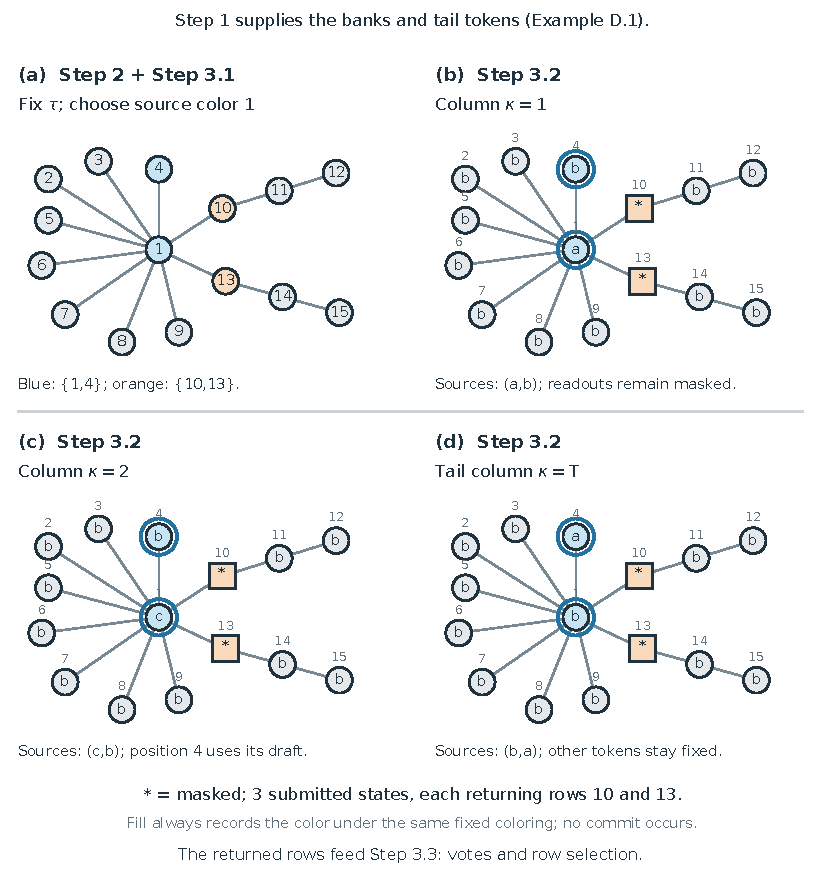
\includegraphics[width=\linewidth]{figures/algorithm_examples_2026-09-18/output/pdf/submissions_2026-09-18.pdf}
 \caption{The coloring and three submitted states of
 \cref{ex:algorithm-submissions-20260918}, labeled by the steps of
 Algorithms~\ref{app:alg:complete-sampler}--\ref{app:alg:packed-screen}.
 All $15$ positions are drawn
 separately at fixed locations. Fill denotes the color under $\tau$;
 square outlines mark masked readouts and double outlines mark sources.
 Small outer numbers are position indices, and inner symbols in
 (b)--(d) are submitted tokens. No vertex is committed by these probes.
 The hidden edges are shown only to explain the construction.}
 \label{fig:algorithm-submissions-20260918}
\end{figure}


\paragraph{TV tests and aggregation.}
Within each coloring, \AlgoBlockRef{aggregate} compares all pairs of
source-column replies at the
same readout; a strict majority across colorings determines each candidate row.
For distinct $i,j\in\ResidualPositions$, when
$\ColorHash{\tau}{i}\ne\ColorHash{\tau}{j}$, define the observable rows
\begin{equation}
 \ProbeObservedRow{\tau}{\kappa}{i}{j}
 :=\OracleRow{\ProbeState{\kappa}{\tau}{\ColorHash{\tau}{i}}
            {\ReadoutChunkOf{\tau}{j}}}{j},
 \quad \kappa\in\ScreenColumnSet,
 \label{app:eq:observed-screen-rows}
\end{equation}
and the observable row family
\begin{equation}
 \ObservedRowFamily{\tau}{i}{j}
 :=\{\ProbeObservedRow{\tau}{\kappa}{i}{j}:
          \kappa\in\ScreenColumnSet\}.
 \label{app:eq:observed-row-family}
\end{equation}
Its TV diameter and the corresponding vote are
\begin{align}
 \ScreenDiameter{\tau}{i}{j}
 &:=\max_{q,q'\in\ObservedRowFamily{\tau}{i}{j}}
      \dTV(q,q'),
 \label{app:eq:observed-screen-diameter}\\
 \ScreenVote{\tau}{i}{j}
 &:=\begin{cases}
 \mathbf 1\{\ScreenDiameter{\tau}{i}{j}>2\RowTVError\},
   &\ColorHash{\tau}{i}\ne\ColorHash{\tau}{j},\\
 0,&\ColorHash{\tau}{i}=\ColorHash{\tau}{j}.
 \end{cases}
 \label{app:eq:screen-vote}
\end{align}
When the colors coincide, the row family and diameter need not be formed.
The vote is set to zero and never refers to an unsubmitted probe.  If
$\MaxBankSize=0$, the screen returns empty rows before forming these objects.

Computing the diameter requires no additional submissions.  It compares
every pair of bank-plus-tail rows, not just each bank row against the tail
column.

For each readout $j$, define the candidate row by
\begin{align}
 \CandidateRow{j}
 &:=\left\{
 i\in\ResidualPositions\setminus\{j\}:
 \sum_{\tau\in\ColoringIndexSet}
 \ScreenVote{\tau}{i}{j}>\frac{\ColoringCount}{2}
 \right\},
 \label{app:eq:provisional-row}
\end{align}

\begin{definition}[Admissible public row selector]
\label{app:def:row-selector}
Let $\ScreenTranscript$ contain the public transcript available when the
screen has finished, including its colors and votes and any retained public
decision-rule state.  A selector $\RowSelector$ is a fixed, terminating,
deterministic measurable rule.  Given $j$, a candidate set
$C\subseteq\ResidualPositions\setminus\{j\}$, the cutoff $\DegreeCutoff$,
and $\ScreenTranscript$, its output has the form
\[
 \RowSelector(j,C,\DegreeCutoff;\ScreenTranscript)
 =
 \begin{cases}
 C,&|C|\le\DegreeCutoff,\\
 C\setminus C_{\mathrm{drop}},&|C|>\DegreeCutoff.
 \end{cases}
\]
On overflow, $C_{\mathrm{drop}}\subseteq C$ is the set of positions that
the rule chooses to remove from these inputs, with
$|C_{\mathrm{drop}}|\ge |C|-\DegreeCutoff$. Thus
$|C\setminus C_{\mathrm{drop}}|=|C|-|C_{\mathrm{drop}}|\le\DegreeCutoff$;
the rule may return fewer than $\DegreeCutoff$ positions, including none.
It makes no oracle submission or commit and reads neither hidden target
information nor unobserved future randomness or oracle replies.
\end{definition}

The returned row $\ScreenRow{j}$ is the output of this selector applied
to $C=\CandidateRow{j}$:
\begin{equation}
 \ScreenRow{j}
 :=\RowSelector\bigl(j,\CandidateRow{j},\DegreeCutoff;
                     \ScreenTranscript\bigr).
 \label{app:eq:returned-row}
\end{equation}
\begin{example*}[Standard top-vote row selector]
The standard choice of $\RowSelector$ for returning $\ScreenRow{j}$ in
\eqref{app:eq:returned-row} orders the positions
$i_1,\ldots,i_{|C|}$ of $C$ by decreasing total vote
$\sum_{\tau\in\ColoringIndexSet}\ScreenVote{\tau}{i}{j}$, breaking ties
by increasing position index. It returns
\[
 \RowSelector(j,C,\DegreeCutoff;\ScreenTranscript)
 =\{i_\ell:1\le\ell\le\min\{\DegreeCutoff,|C|\}\}.
\]
Thus it keeps all of $C$ when $|C|\le\DegreeCutoff$ and otherwise removes
the positions ranked after $\DegreeCutoff$. The empty input gives the
empty set. Taking $C=\CandidateRow{j}$ gives the standard returned row
$\ScreenRow{j}$.
\end{example*}
The size cap alone would not suffice: deleting a candidate from a
nonoverflowing row can destroy low-degree exactness.
When $\MaxBankSize=0$, every returned row is defined to be empty.

\begin{proposalcontext}{Alternative overflow rule}
Returning $\emptyset$ on overflow is another admissible selector.
The standard sampler uses top-vote selection; the invariance proposition
compares the guarantees of these rules, not their realized performance.
\end{proposalcontext}

Given its inputs, public transcript, and the frozen oracle,
\cref{app:alg:packed-screen} is deterministic; the full decision rule in \cref{app:alg:complete-sampler}
supplies its color family in \AlgoBlockRef{draft}.
It expands \MainAlgoBlockRef{screen} of
Algorithm~\ref{main:alg:upper-bound-sampler}.
Within \AlgoBlockRef{screen}, \AlgoBlockRef{aggregate} computes votes
after each chunk's probes, then forms and selects rows after all colorings.

\begin{algorithm}[H]
\caption{Packed color screen with a fixed draft}
\label{app:alg:packed-screen}
% Retain the former main-text screen label as an alias for archived references.
\label{main:alg:packed-screen}
\begin{algorithmic}[1]
\Require $\History$, $\PreprocessData$, $\DraftFiller$, a color set $\ColorSet$, and a family
  $(\ColorHash{\tau}{\cdot})_{\tau\in\ColoringIndexSet}$,
  $\DegreeCutoff,\ChunkCount$, read access to $\FrozenOracle$,
  $\RowSelector$, and the current public transcript $\ScreenTranscript$
\Ensure $(\ScreenRow{j})_{j\in\ResidualPositions}$; the history is unchanged
\If{$\MaxBankSize=0$ or $\ResidualPositions=\emptyset$}
  \State \Return $(\emptyset)_{j\in\ResidualPositions}$ without a counterfactual submission
\EndIf
\State Initialize all votes in \ref{app:eq:screen-vote} to zero
\For{$\tau\in\ColoringIndexSet$}
  \Statex \AlgoBlockTarget{chunks}
  \State Form the color classes and current readout chunks by
    \ref{app:eq:color-class}--\ref{app:eq:readout-chunks}
  \For{each nonempty readout chunk
      $\mathcal C=\ReadoutChunk{\tau}{\ReadoutColorValue}{m}$}
    \Statex \AlgoBlockTarget{probes}
    \For{$\kappa\in\ScreenColumnSet$}
      \For{$\SourceColorValue\in
             \ColorSet\setminus\{\ReadoutColorValue\}$}
        \State Submit $\ProbeState{\kappa}{\tau}{\SourceColorValue}{\mathcal C}$
          and read all rows $j\in \mathcal C$
      \EndFor
    \EndFor
    \Statex \AlgoBlockTarget{aggregate}
    \State Form the row-family diameters and votes for all
      $i\in\ResidualPositions\setminus\{j\}$ and $j\in \mathcal C$ using
      \ref{app:eq:observed-row-family}--\ref{app:eq:screen-vote}
  \EndFor
\EndFor
\Statex \AlgoBlockHeading{aggregate} (continued)
\State Form the candidate rows by \ref{app:eq:provisional-row}
\State Append the current screen's replies, colors, and votes to $\ScreenTranscript$
\State Apply the public selector by \ref{app:eq:returned-row}
\State \Return $(\ScreenRow{j})_{j\in\ResidualPositions}$
\end{algorithmic}
\end{algorithm}

Every bank- or tail-column state is a noncommit counterfactual submission, and the
submitted states agree with $\History$ on $G$.  One submitted state returns all
rows indexed by its readout chunk and contributes one to
$\CounterfactualQueries$, regardless of $|\mathcal C|$
(\textcolor{red}{\cref{app:def:resources}}). The
tail-column reply for a fixed $(\tau,\mathcal C,\SourceColorValue)$ is reused in the
diameter computation for that source color, not across different source colors.

\subsection{Roles of the construction and proof route}
\label{app:algorithm-proof-route}

\textcolor{red}{The overview in \cref{app:upper-proof-overview} maps the steps above
to their structural, resource, and error guarantees. It also gives the proof
routes for both accuracy cases and their specialization to
\cref{main:thm:upper-curve}.}

\begin{proposalcontext}{Scope of cycle repair}
Cycle repair avoids an immediate all-residual product commit merely because
the terminal estimate has a cycle. A repaired forest need not contain every
true residual edge. The guarantees still charge failed-screen paths to the
screen-failure budget; they do not assert an accuracy improvement over the
one-batch alternative.
\end{proposalcontext}
